% Two sided means the left and right margins are different sizes and they alternate every page. 
% If your document is printed to be book or spiral bound this allows for a thick spine to not 
% eat into the space for your page content. 
\documentclass[11pt, a4paper, twoside, openright]{custard}

% All imports, packages, and configuration in here. 
% Your document should be about content so we abstract away the styling rules and tools we are using. 
%% Here you can specify new commands and environments that you intend
%% to use. Using commands can make your document easier to write, read
%% and be more consistent.

\usepackage[linesnumbered,ruled]{algorithm2e}
\DeclareMathOperator*{\argmin}{arg\,min}

\usepackage{appendix}
\usepackage{textcomp}
\usepackage{setspace}
%\usepackage[document]{ragged2e}
\usepackage{verbatim}
\usepackage{multirow}
\usepackage{multicol}
\usepackage{booktabs}
\usepackage{enumitem}
\sloppy
\usepackage{graphicx}
\usepackage{threeparttable}
\usepackage{epsfig}
\usepackage{epstopdf}
\usepackage{float}
\usepackage{enumitem}
\usepackage{cite}
\usepackage[export]{adjustbox}
\usepackage{algorithmic}
\usepackage[nohyperlinks,printonlyused]{acronym}
\usepackage{amsmath}
\usepackage{amsfonts}
\usepackage{array}
\usepackage{tabularx}
\usepackage{longtable}
\usepackage{times}
\usepackage{amssymb}
\usepackage{hhline}
\usepackage{color}
\usepackage{soul}
\usepackage{colortbl}
\definecolor{Gray}{gray}{0.85}
\usepackage{rotating}
\usepackage{fix2col}
\usepackage{pdflscape}
\usepackage{pdfpages}
\usepackage{stmaryrd}
\usepackage[export]{adjustbox}
\usepackage{bbm}
\usepackage{relsize}
\usepackage{xfrac}
\usepackage{bibentry}

%\usepackage{refcheck}

%watermarking
\usepackage[english]{babel}
\usepackage{tikz}

%% Uncomment the following line for hyper links - not recommended for printing
\usepackage[colorlinks, linkcolor=, anchorcolor=, citecolor=, filecolor=, menucolor=, runcolor=, urlcolor=]{hyperref}

\setcounter{tocdepth}{1}
%\setcounter{minitocdepth}{3} 
\linespread{1.31}

\newcommand\litem[1]{\item{\bfseries #1:\enspace}}

\interdisplaylinepenalty=2500

\newcolumntype{L}[1]{>{\raggedright\let\newline\\\arraybackslash\hspace{0pt}}m{#1}}
\newcolumntype{C}[1]{>{\centering\let\newline\\\arraybackslash\hspace{0pt}}m{#1}}
\newcolumntype{R}[1]{>{\raggedleft\let\newline\\\arraybackslash\hspace{0pt}}m{#1}}

\renewcommand{\thefootnote}{\fnsymbol{footnote}}
\setlength{\LTpre}{-10pt}\setlength{\LTpost}{-30pt}%
\newcommand{\oiint}{\begin{picture}(0,0)(-10,-2)\put(0,0){\oval(12,8)}\end{picture}\iint}
\renewcommand{\mathbf }{\boldsymbol}

\def \eg{e.g.\ } % Allows you to write \eg in LaTeX instead of typing e.g. so that every single one will be formatted the same.
\def \Eg{E.g.\ } % Define some other common variants. If you later want to change one of these definitions, 
\def \ie{i.e.\ } % it will update all the usages throughout the document.
\def \Dr{Dr.\ }
\def \vs{vs. }
\def \etal{\emph{et al.\ }} 
\def \sota{state-of-the-art }
\def \handcrafted{hand-crafted }

\usepackage{listings,lstautogobble}
\usepackage{sourcecodepro}
\pdfmapfile{=SourceCodePro.map}
\lstset{
	xleftmargin=0.5cm,frame=tlbr,framesep=4pt,framerule=0.5pt,
	language=,
	upquote=true,
	columns=fixed,
	tabsize=2,
	extendedchars=true,
	breaklines=true,
	numbers=left,
	numbersep=10pt,
	basicstyle=\ttfamily\scriptsize,
	numberstyle=\tiny,
	stringstyle=\ttfamily,
	captionpos=b,
	showstringspaces=false,
	autogobble=true
}

\usepackage[font=small,skip=10pt]{caption} %,format=hang
%\usepackage[labelformat=simple]{subcaption}
\usepackage[labelformat=simple]{subfig}
%\captionsetup[figure]{format=hang}
%\captionsetup[lstlisting]{format=hang}
\renewcommand{\thesubfigure}{\Alph{subfigure}.}

\renewcommand{\thefootnote}{\arabic{footnote}}

% Use IEEEtran citation style. 
\bibliographystyle{IEEEtran} 

\def\samplefont#1{%
    % set font style and save name
    #1\edef\savedname{\fontname\font}%
    % print small sample
    {\leavevmode\tt\hbox to 1in{\savedname:\hss}}%
    abcxyz ABCXYZ 123\par
}

\begin{document}
	
% The custom data for Swansea University and your degree name.
% The \protect\\ command forces a new line in the title which might be otherwise overriden by the template
	\title{Parallel Counting for the N-Queens Problem}
	\author{Ben Howard\protect\\{\normalsize 1905021}}
	\awardinginst{Swansea University}
	
% Comment / uncomment your degree type as needed.
	\degree{Bachelor of Science} 
	%\degree{Master of Science}
	%\degree{Doctor of Philosophy}
	
% Institution details and logo
	\department{Department of Computer Science}
	\university{Swansea University}
	\unilogo{graphics/swansea.png}
	
% Hard code the date or allow the LaTeX compiler to fill it in whenever you recompile the document.
	\date{\today}
	
% Build the title and declaration pages, and pad the document so the text starts on a right hand book page.
% Page numbering is in roman numerals until the first page of an actual chapter which resets numbers 
% starting from 1 at that point. 
	\frontmatter%
	\maketitle
	\declaration
	\cleardoublepage
	
% Most books and theses have a brief foreword or dedication. 
	\begin{vplace}[0.7]
		\begin{large}
			\begin{center}
				\textit{I would like to dedicate this work to the Hypnotoad.\\All glory to the Hypnotoad.}
			\end{center}
		\end{large}
	\end{vplace}

% Abstract comes before the contents page.	
	\begin{abstract}
		\vspace{-2em}
		\setcounter{page}{1}
		
		Put abstract here
	\end{abstract}
	
% A long form dedication. 
	\begin{Acknowledgements}
		This is an opportunity to acknowledge and thank those who have supported you throughout your studies. Friends and colleagues who you have studied alongside, your families, and your mentors within the department are the usual suspects. 
	\end{Acknowledgements}
	
% Build the table of contents page.
	\tableofcontents*
	 
% Optionally you can make a bank of known acronyms in acronyms.tex that you can call on throughout your document.
	%\input{acronyms} 
	
% For long documents like a Doctoral thesis you should include a list of tables and figures throughout 
% your document. This is uses a shortened version of each table and figures caption and enumerates all 
% of them with their table or figure number. This is automatic, you do not need to modfy it if you do use it.
	\setlength{\columnsep}{10pt}
\newpage
\listoftables
\mtcaddchapter 
\newpage
\listoffigures
\mtcaddchapter  
	
% Reset numeric page numbering from page 1
	\mainmatter%

% Insert the code for each of your chapters
	\chapter{Introduction}\label{chap:intro}
The N-Queens problem initially started out as the eight queens puzzle. First proposed by chess composer Max Bezzel in 1848 to renowned chess players all over Germany\cite{bezzel}. The aim of the puzzle was to place eight queens on the standard eight by eight chessboard. The queen can move vertically, horizontally and diagonally in any direction on the board and thus is the most valuable chess piece on the board excluding the king. It's troublesome to find a single solution to the problem, but the real goal is to find every possible solution. The eight queens puzzle was fully solved in 1850 by Franz Nauck who successfully found all 92 solutions\cite{Nauck}. With the succession of this solution, many chess composers began to theorise about non-standard chessboards.
	
With larger sizes of boards looking to be solved, the problem transformed in the N-Queens puzzle. The rules are identical to the eight queens puzzle although the number of queens to place scales with the size of the board. As mathematicians and chess players began to solve for larger board sizes, they found that number of solutions would increase dramatically. There exists solutions for all natural numbers except for \(n = 2\) and \(n = 3\)\cite{hoffman}. As in the eight queens puzzle, finding a single non-trivial solution isn't the real goal, but finding all possible for a certain board size. 
    
Interest in computing this problem was popularised by Dijkstra in 1971 when he included in his paper "A short introduction to the art of programming"\cite{dijstra}. It became a common exercise for backtracking in many artificial intelligence and constraint programming textbooks. Backtracking can provide a complete solution to the N-Queens problem with all solutions found to a given board size. As well as being an exercise in artificial intelligence and constraint programming, the N-Queens problem also lends itself to parallel programming. 
    
The N-Queens problem is a perfectly parallel problem which makes it trivial to implement into a parallel system. This is because there is very little effort in splitting this problem into multiple parallel tasks. We can achieve this by running a solving algorithm on a partly complete board. The simplest option would be to place a queen in each position of a row or column, this would split the workload into eight distinct tasks that could be solved simultaneously. We can produce more parallel tasks by solving the problem to set depths. The exploration of solving the N-Queens problem through parallelism will be the focus of this paper.   
    
    
\section{Aims and Objectives}                                                           \label{sec:intro_aims} 
The increasing importance of parallel computing has never been clearer. With the exponential growth of processing and network speeds, parallel computing has become a necessity. Examples of parallel computing can be seen everywhere in today’s society from smartphones with multicore processors, to medical research using parallel systems to simulate protein sequence alignment\cite{li2003clustalw}. It is an industry that will keep growing alongside the computation of data as a whole. 
        
High Performance Computing (HPC) is the ability to process data and perform complex calculations at high speed and is a topic I haven't worked with. With that, the bulk of my project will be spent designing and implementing algorithms to run on parallel systems. I will be able to test my code on my personal computer as it has multiple cores. There are many existing N-Queens algorithms that have been executed on HPC's before, I intend to learn how these work and how they were implemented. 
        
Obviously the ultimate aim for this project and most N-Queen problem papers is to calculate the solution to the 28-Queens problem. Although this is an incredibly unlikely aim for myself due to the lack of time and resources I have available at my disposal. Top500 is a project that aims to maintain HPC statistics and ratings on a bi-yearly basis\cite{top500}. As of November 2021 the highest rated HPC is the Japanese supercomputer Fugaku with it's peak performance sitting at over a exoflop and some seven million cores\cite{top500fug}. Many of the current projects looking to solve the 28-Queens problem comfortably sit in the Top500 with access to these systems for prolonged periods of time. Also many of these projects have a team of academics looking to optimise every aspect of the operation. With my limited resources and access to high performance computers, alongside my set time frame, this will merely be an introduction into the world of parallel computing and thus my aims will be set accordingly. 
\begin{description}
\item[Aim 1] -- To implement a parallel N-Queens algorithm on a HPC.
\item[Aim 2] -- To measure and collect the speed and accuracy of the algorithm.
\item[Aim 3] -- Use the speed and accuracy data collected to improve and redesign the algorithm.
\item[Aim 4] -- Summarize my findings and compare the various algorithms and methods implemented.
\item[Aim 5] -- To correctly calculate the highest value of \(n\) and to compare my results to other projects.  
\end{description}
These aims were set in order to not only achieve the bare minimum of implementing a parallel algorithm on a HPC but analyse it in order to improve it. The improvement and speed of algorithms is an important part of this project so a large period of time will be dedicated to analysing and improving these algorithms. I understand with my limited resources I will be unable to produce any groundbreaking research but will put emphasis on the learning process throughout this project to help others who have similar goals. 
	\chapter{Background}\label{chap:background}
\section{N-Queens}\label{sec:background_nqueens} 
Calculating the N-Queens problem has been a long tradition the computer science field and has been famously used in examples of backtracking\cite{golomb}, constraint satisfaction\cite{nadel1989constraint} and permutation generation\cite{swarm}.
		
Although the N-Queens problem is not a constraint satisfaction problem, it can be naturally formulated as one\cite{nadel1990representation}. Brute force techniques are mostly overlooked with the large number of possible arrangements and the low number of possible solutions. Although as there are set constraints on where the queen can be placed, we can use shortcuts in order to reduce the number of possible arrangements. For example limiting a single queen to a row, we reduce the total number of possible arrangements to \(8^8\). We could then blindly place a queen in each column/row and although this is still a very poor algorithm, it is one of the most efficient brute force algorithms. 
		
% It's often a good idea to generate the LaTeX code for tables (python script or similar) so that if you rerun your code you don't have to typeset your results again by hand!
\begin{table}[H]
\centering
\begin{tabular}{|l||l|l|}
\hline
n  & Fundamental            & All                     \\ \hline \hline
1  & 1                      & 1                       \\ \hline
2  & 0                      & 0                       \\ \hline
3  & 0                      & 0                       \\ \hline
4  & 1                      & 2                       \\ \hline
5  & 2                      & 10                      \\ \hline
6  & 1                      & 4                       \\ \hline
7  & 6                      & 40                      \\ \hline
8  & 12                     & 92                      \\ \hline
9  & 46                     & 352                     \\ \hline
10 & 92                     & 724                     \\ \hline
11 & 341                    & 2,680                   \\ \hline
12 & 1,787                  & 14,200                  \\ \hline
13 & 9,233                  & 73,712                  \\ \hline
14 & 45,752                 & 365,596                 \\ \hline
15 & 285,053                & 2,279,184               \\ \hline
16 & 1,846,955              & 14,772,512              \\ \hline
17 & 11,977,939             & 95,815,104              \\ \hline
18 & 83,263,591             & 666,090,624             \\ \hline
19 & 621,012,754            & 4,968,057,848           \\ \hline
20 & 4,878,666,808          & 39,029,188,884          \\ \hline
21 & 39,333,324,973         & 314,666,222,712         \\ \hline
22 & 336,376,244,042        & 2,691,008,701,644       \\ \hline
23 & 3,029,242,658,210      & 24,233,937,684,440      \\ \hline
24 & 28,439,272,956,934     & 227,514,171,973,736     \\ \hline
25 & 275,986,683,743,434    & 2,207,893,435,808,350   \\ \hline
26 & 2,789,712,466,510,280  & 22,317,699,616,364,000  \\ \hline
27 & 29,363,495,934,315,600 & 234,907,967,154,122,000 \\ \hline
\end{tabular}
\caption{\label{tab:solutions}Total number of solutions for given \(n\) size.}
\end{table}
		
% [H] means put the figure HERE, directly when you input this code.
\begin{figure}[H]
	\centering

% We set the width of the figure based on the width of one line of text on the page. 
% The value can be tuned to any value in [0.0, 1.0] to scale the image while maintaining its aspect ratio.
	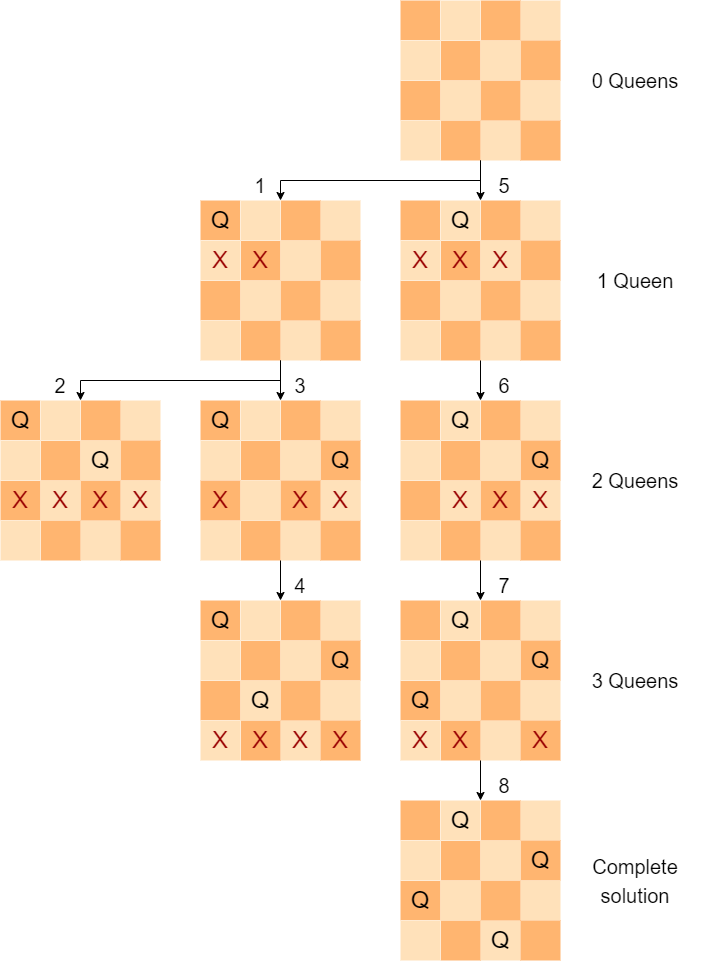
\includegraphics[width=0.5\linewidth]{./graphics/n4_backtracking.drawio.png}
	
% Caption is defined with a short and long version. The short version is shown in the 
% List of Figures section, and the long version is used directly with the figure. 		
	\caption[A N-Queens backtracking algorithm shown to get one solution for \(n = 2\)]{A N-Queens backtracking algorithm shown to get one solution for \(n = 2\)}
	
% For figures label should be defined after the caption to ensure proper figure numbering.
	\label{fig:n4_backtracking}
	
\end{figure}
Backtracking the N-Queens problem is a process of systematically placing queens and when we get to a position where no more queens can be placed, we backtrack to the previous placement and try the next available placement. In \ref{fig:n4_backtracking} we can see a full run through of the backtracking algorithm to a single solution. The algorithm will start by placing a queen in first available spot in the first row. It then moves onto the second row looking to place, there are two available locations, it will pick the furthest to the left first, although as it goes to place the third queen, it will find no available placements. It will then remove the last placed queen and place on the next available location. This continues until a solution is found although at this point the algorithm can return the board or increment the total number of solutions and then continue looking for solutions. This algorithm is complete and thus will find all possible solutions. This solution essentially creates a tree with the further you descend the tree, the more queens are placed on the board. 
		
An idea to compose a solution to the N-Queens problem by using the solutions to smaller n sizes was introduced by Ahrens\cite{ahrens}. Although the idea was limited by the fact it was only able to produce a strict class of solutions. Therefore it was a non complete solution unlike search based solutions.
		
Artificial Intelligence can also be used to solve the N-Queens problem\cite{sosic1990polynomial}. We can begin with a randomly generated board such as one where a single queen is placed in each row/column like in the brute force example. From this point we can count the number of attacks between each of the queens and attach values to the queen placements. We can use heuristics that uses this information to improve the placement of the queens and then analysing the placements again. The algorithms speed and efficiency is heavily based of the initial configuration of queens. This is a greedy algorithm meaning it will select the best option available at the moment. This isn't ideal for generating all solutions to the N-Queens problem as greedy algorithms are not complete.
		
The N-Queens algorithm is an NP-complete as well as \#P-complete algorithm. For a problem to be NP-complete it has to be in the set NP meaning it can be brute forced in polynomial time and can be reductable to a simulate every other NP problem. For the problem to be \#P it must belong in a class of problems that can be solved in polynomial time by a deterministic Turing machine.
		


% [H] means put the figure HERE, directly when you input this code.
\begin{figure}[H]
	\centering
	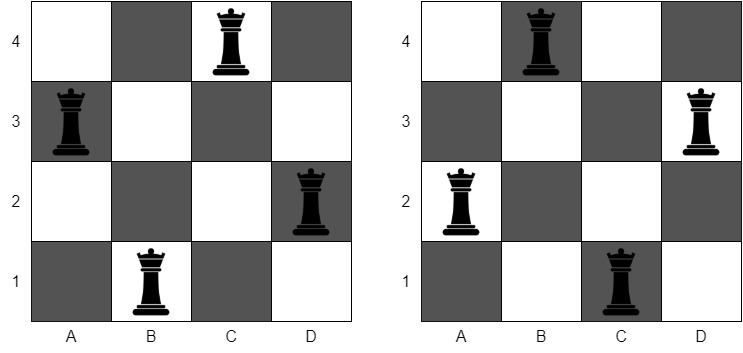
\includegraphics[scale=0.4]{graphics/symmetry.jpg}
	\caption{Symmetry between two $4\times 4$ n queen solutions.}
	\label{fig:symmetry}
	
\end{figure}
		
When looking to find all solutions for a certain size \(n\), we can use the symmetry of the chess board to our advantage. As you can see in figure \ref{fig:symmetry}, we were able to derive a second solution to a four queen problem by reflecting the known solution. Although we have the two solutions to the 4 queen problem, only one solution is distinct and the other is a reflection/rotation. We call the distinct solution a fundamental solution. Each fundamental solution can have up to eight variant solutions (including it's original) by rotating 90, 180 and 270$^{\circ}$ and then reflecting each rotation on a fixed axis. This allows us to provide two values for the total number of solutions, the fundamental number of solutions and the total number of solutions. As you can see in table \ref{tab:solutions} the number of solutions increases dramatically with each increase of \(n\). \(n=27\) is the highest order board that has been completely enumerated. 

\section{Related Work}\label{sec:background_relatedwork} 

Given the N-Queens extensive history, it has gathered significant amount of study either looking to increase the known solutions or find real world applications. In 1986 the New Mexico State University Department of Computer Science released a paper detailing an N-Queens algorithm that could run concurrently\cite{Silver}. It used the programming language Modcap which is a block-structured function-based expression language. Although they did not have access to a parallel computer, after simulating how would run on a serial machine they came to the conclusion that it could run 300 times faster on a parallel system over serial execution. 

The next documented evidence of parallelization of the N-queens problem was in 2004 by The University of Electro-Communications in Tokyo\cite{kenji}. This team successfully calculated the total number of solutions to the 24-Queens problem on a 34-node PC cluster. A total of 227,514,171,973,736 solutions were calculated and took the cluster 22 days to calculate. The backtracking algorithm they used was heavily based off Jeff Somer's C program which I will go into detail about later in this paper. They designed a sequential program that is parallelized using MPI (Message Passing Interface). MPI allows for the distributed memory communication of nodes in a parallel system. I will be going into more detail about MPI later in this paper. 

Later in 2004 another project surfaced that aimed to solve the 25-queens problem\cite{caromel}. The research group was a group of individuals from the University of Nice Sophia Antipolis. This was achieved by using the spare CPU cycles of 260 machines using the ObjectWeb ProActive library. The total computation time was over 4,444hrs or 185 days. Although the accumulated computation time was 464,344hrs or over 53 years. The total number of solutions calculated is 2,207,893,435,808,352 and they were the first to do so. This really shows the power of parallel computing as they were able to execute the necessary tasks over 100 times quicker than on a serial system. 

The \(n = 26\) and \(n = 27\) were both first solved by TU Dresden (Technical University of Dresdon, Germany) in 2009 and 2016 respectively\cite{thomas}. To achieve this they used an FGPA (Field-Programmable Gate Array) implementation. FPGA's allows for a programmable hardware circuit that can be used to optimise a chip for a particular workload. The solution for \(n = 26\) was a massive 22,317,699,616,364,044 total solutions. It took another 7 years of research from various institutions to solve \(n = 27\) of the n-queens problem. It was again solved using FGPA's but these were greatly optimised and they exploited the use of symmetries to reduce the amount of computation drastically. This solution is where the record stands today with \(n = 28\) which will most likely have over (\(10^{18}\)) solutions.

The N-Queens algorithm is often studied as a "mathematical recreation" although there has been several real world applications directly linked to N-Queens solutions. Erbas, Tanik and Nair introduced a memory storage concept for parallel memory system making use of the N-Queen solutions allowing conflict free access to rows, columns and diagonals\cite{erbas1993circulant}. Tanik also went onto describe a method for deadlock prevention through the use of N-Queens. solutions\cite{tanik1978graph}. It has also been noted the N-Queens solutions could be used for VLSI (Very Large Scale Integration) testing and traffic control\cite{sosic1990polynomial}as well as image processing\cite{wang2006fast}. 

\section{Parallelisation}\label{sec:background_parallelisation } 
Parallel computing refers to the process of breaking down large computational problems into smaller parts that can be executed simultaneously across multiple processing cores that may communicate    via a shared memory. We can call these smaller parts concurrent processes. Concurrent computing is the set of serial (or sequential) programs that have the ability to run in parallel\cite{ben2006principles}. The aim of parallel computing is to increase the available computational power for problem solving. The problem is first split up into discrete parts that may be solved concurrently. Each of these parts are then broken down into a series of instructions that may run serially. Each of these parts are run on separate processing units simultaneously. A control mechanism can be put in place to control what processing units execute what parts. Although parallel computing now seems like the solution to all, in many situations serial computing is quicker and more efficient than parallel computation. Parallel slowdown is a phenomenon in which more time is spent communicating with other computers than processing data causing a communication bottleneck, slowing down the system. As long as a computational problem can be split into multiple discrete parts that may run serially and can be solved without parallel slowdown, parallel computing will always be the better option.

Communication between the parallel processes is not always necessary. As stated earlier, the N-Queens problem is perfectly parallel meaning it is trivial to split into the parallel tasks. For this the only communication needed will be to add up the total number of solutions at the end of execution.

In 1992 at the Supercomputing Conference the Message Passing Interface (MPI) forum was created with the intention of creating a standardisation for message passing between parallel processes\cite{gropp1996high}. With the assistance of more than 80 people from 40 organisations, version 1 of the MPI standard was released in 1994\cite{snir1998mpi}. MPI became a communication protocol for programming in parallel with each parallel process executing in isolation. Each process will have it's own dedicated memory space that the other processes do not have access to. Both process to process and collective communication is supported in the protocol. It has become the standard convention for communication among processes in distributed memory systems. 

The OpenMP API used in Fortran, C and C++ supports shared memory parallel programming. It can be used to develop parallel applications that make use of the same memory space. It can be seen as multiple processes running together sharing each others memory and resources\cite{chandra2001parallel}. Shared memory has it's benefits over distributed memory systems with shared memory being a lot easier to parallelize compared to distributed memory.    

I will be using MPI instead of OpenMP in my project for the reason that limited parallel communication is needed. If I used OpenMP, I would have to be careful with my memory management and process timing otherwise I could run into deadlock, race conditions and resource starvation\cite{ben2006principles}. I will be using the MPICH implementation of the MPI standardization\cite{gropp1996user}. This allows me to create MPI executables in Fortran77, Fortran90, C and C++. I can then execute the program and specify the number of processors the program will use. 

With that choice, I needed to decide on what language I would program this algorithm in. After doing some research I found that Fortran was much slower in parallel environments compared to C and C++ and gave a better speedup with the increase of cores\cite{young2016openmp}\cite{cary1997comparison}. C++ is a super set of C meaning it is based upon C and C++ has additional functionality over C. This includes modern OOP (Object Oriented Programming) concepts such as encapsulation and inheritance. When Bjarne Stroustrup created C++, it was evolved from C and nicknamed "C with classes"\cite{stroustrup1996history}. As I am familiar with OOP languages and am looking the set of OOP languages I understand, I will be developing this program in C++ over C and Fortran.  

This algorithm will require storage of the current board state, or more specifically the queen locations. The first obvious choice would be a two dimensional matrix of Boolean's. We could represent 0 as and empty board location and 1 as a queen placement.  
\begin{figure}
    \centering
    \begin{pmatrix}
    0 & 0 & 0 & 0 & 1 & 0 & 0 & 0\\
    0 & 1 & 0 & 0 & 0 & 0 & 0 & 0\\
    0 & 0 & 0 & 1 & 0 & 0 & 0 & 0\\
    0 & 0 & 0 & 0 & 0 & 0 & 1 & 0\\
    0 & 0 & 1 & 0 & 0 & 0 & 0 & 0\\
    0 & 0 & 0 & 0 & 0 & 0 & 0 & 1\\
    0 & 0 & 0 & 0 & 0 & 1 & 0 & 0\\
    1 & 0 & 0 & 0 & 0 & 0 & 0 & 0\\
    \end{pmatrix}
    \caption{A solution the 8-Queens problem represented as a Boolean matrix}
    \label{fig:n8matrix}
\end{figure}




	
% Formatting citations properly when they are rendering incorrectly in your PDF can be fiddly,
% especially when punctuation and international characters are involved. Sometimes multiple re-compilations
% are needed in addition to clearing temporary auxiliary files to see your changes in your document.
% Insert the bibliography using citations contained in the file citations.bib
	\bibintoc%
	\bibliography{citations} 
	
% In the appendix you might include a full code listing for an implemented algorithm that you showed a 
% small chunk of in one of your chapters. If you have extra graphs for ablation style experiments you 
% might enumerate them within the appendix and use \label{name} and \ref{name} to automatically insert 
% the correct section locations when you talk about them in your chapters.
% Within appendix.tex you should use chapters as the top level section dividers.
	%\appendix
	%\addappheadtotoc
	%%\chapter{Implementation of a Relevant Algorithm}
%\label{app:implementation_algorithm}

% Code listings should live in a code file, not embedded directly into your LaTeX code!
%\lstinputlisting[language=c, label={lst:c_hello_world}, caption={An implementation of an important algorithm from our work.}]{./listings/hello_world.c}

%\chapter{Supplementary Data}
%\label{app:supplementary_data}

%The results of large ablative studies can often take up a lot of space, even with neat visualization and formatting. Consider putting full results in an appendix chapter and showing excerpts of interesting results in your chapters with detailed analysis. You can use labels and references to refer the reader here for the full data.

	
\end{document}